\section{RF Link budget} \label{an:rf-link-budget}
\newcommand{\cod}{SB1FS-COM-}
% In this appendix RF link budgets are presented for \textbf{EWC30-FM1} and \textbf{EWC30-FM2}. The \textbf{"main line"} refers to the RF path that goes from the Transmitter to the Receiver.
% The \textbf{"instrumentation line"} refers to the RF path that goes 
% from an output of a directional coupler to the PXI or PXA spectrum analyzer.\\

% The summary tables show the power value received by the receiver under different conditions.
% The nominal condition corresponds to the budget shown in the "main line" table.
% The Maximum Level condition corresponds to the configuration that allows to achieve the highest power in the receiver or instrument.
% It is observed that the maximum values achieved do not exceed the values accepted by the receivers or instrument. \\
 
% The tables show components highlighted in red, they are not characterized, 
% thus the indicated attenuation is an estimate. When the characterization 
% of the components is carried out, the link calculations will be updated. 
% The changes in the expected levels are in the order of tenths of dB. \vspace{15mm}

This appendix presents link budgets for \textbf{EWC30-FM1} and \textbf{EWC30-FM2} 
tests and has three cases.
The first case uses the setups showed in figures \ref{fig:setup_xband_funcional} and  \ref{fig:data-setup1}.
The second case use the setup showed in figure \ref{fig:data-setup1} and 
the third case use the setup showed in figure \ref{fig:data-setup2}. This budgets are performed with the 
GS-GSE-FM~(R). The link budget for the first case is presented in tables \ref{tb:Data_DWL1} and 
\ref{tb:Data_DWL2} this applies to \textbf{\cod{F-012-02} Aliveness and Functional Test}, 
\textbf{\cod{P-013-02} \TestPerfRFPXA}, \textbf{\cod{P-013-03} \TestPerfCCDF}, 
\textbf{\cod{P-013-04} \TestPerfFreqS}, \textbf{\cod{P-013-05} \TestPerfCWPhaseN} and 
\textbf{\cod{P-013-06} \TestPerfFilterVector} tests. In all these tests, except the first and the last,
 the GS-GSE-FM~(R) operate as a load and the instrumentation line is connected to the CEGSE. 
 The link budget for the second case is presented in tables \ref{tb:Data_EBN0FM1} and \ref{tb:Data_EBN0FM2} 
 this applies to \textbf{\cod{P-013-07} \TestPerfBer} test. 
In this test, the DUT power signal is connected to the X-Band port of \gse-FM (R), the Noise generator 
(TestBed) is connected to the other X-Band port. The link budget for the third case is 
presented in tables \ref{tb:Data_DSNFM1} and \ref{tb:Data_DSNFM2}, 
and applies to \textbf{\cod{P-013-08} \TestPerfSpuriousDSN}
test. In this test, the DUT power signal is connected to Instrument Port.\\
\vspace{0.5cm}

Related to second case, X-Band Downlink budget is dimensioned in order to obtain Eb/N0 specified 
values (6dB to 2dB) as shown in \refAD{test-spec-XB}, thus, the setup showed in figure 
\ref{fig:data-setup1} is obtained in order to achieve minimum specified Eb/N0 values. Eb/N0 
budget shows that it can obtain Eb/N0 values from $\approx$ 6dB to $\approx$2dB setting Noise Density level 
from -103dBm/Hz to -99dBm/Hz, respectively. For this case Eb/N0 required are adjusted only 
from Cortex HDR-XXL of TestBed. %Table \ref{tb:Data_ebn0} shows Eb/N0 approximation obtained 
%at the input ports of GS-GSE-FM (N) with -95dBm/Hz Noise density.\\
\vspace{0.5cm}


Summary tables are presented at the end of budgets showing attenuation values of components 
that can be configured, and power values received by the receivers under different conditions. 
The nominal condition corresponds to the budget shown in the "main line" table. The Maximum 
Level condition corresponds to the configuration that allows to achieve the highest RF power
 in the receivers and the PXI or PXA as applicable. For all cases are observed that in conditions of minimum 
 attenuation and maximum gain, the maximum power values achieved not exceed the value accepted
  by the Data Demodulator or instrument.\\
  \vspace{0.5cm}

For all cases, PXA is set to measure DUT power TX levels, therefore, it is configured with a 
references level offset.\\
\vspace{0.5cm}
The tables show components highlighted in red, they are not characterized, 
thus the indicated attenuation is an estimate. When the characterization 
of the components is carried out, the link calculations will be updated. 
The changes in the expected levels are in the order of tenths of dB.

%
%        \subsection{TM Downlink}
%\begin{table}[H]
%\centering
%	\includegraphics[page=1, scale=0.8, trim=0cm 4cm 0cm 0cm, clip ]
%	{tables/Ensayos COMM-SS Link Budget - S-Band TM Downlink.pdf}\\
%	\caption{COMM-SS Link Budget - S-Band TM Downlink.} \label{tb:TM_DWL}
%\end{table}
%    \subsection{TC Uplink}
%\begin{table}[H]
%\centering
%	\includegraphics[page=1, scale=0.8, trim=0cm 3cm 0cm 0cm, clip ]
%	{tables/Ensayos COMM-SS Link Budget - S-Band TC Uplink.pdf}\\
%	\caption{COMM-SS Link Budget - S-Band TC Uplink.} \label{tb:TC_UPL}
%\end{table}

%\subsection{Data Downlink}
\begin{table}[H]
	\centering
	\caption{EWC30-FM1 Link Budget - X-Band Data Downlink - case 1.} \label{tb:Data_DWL1}
	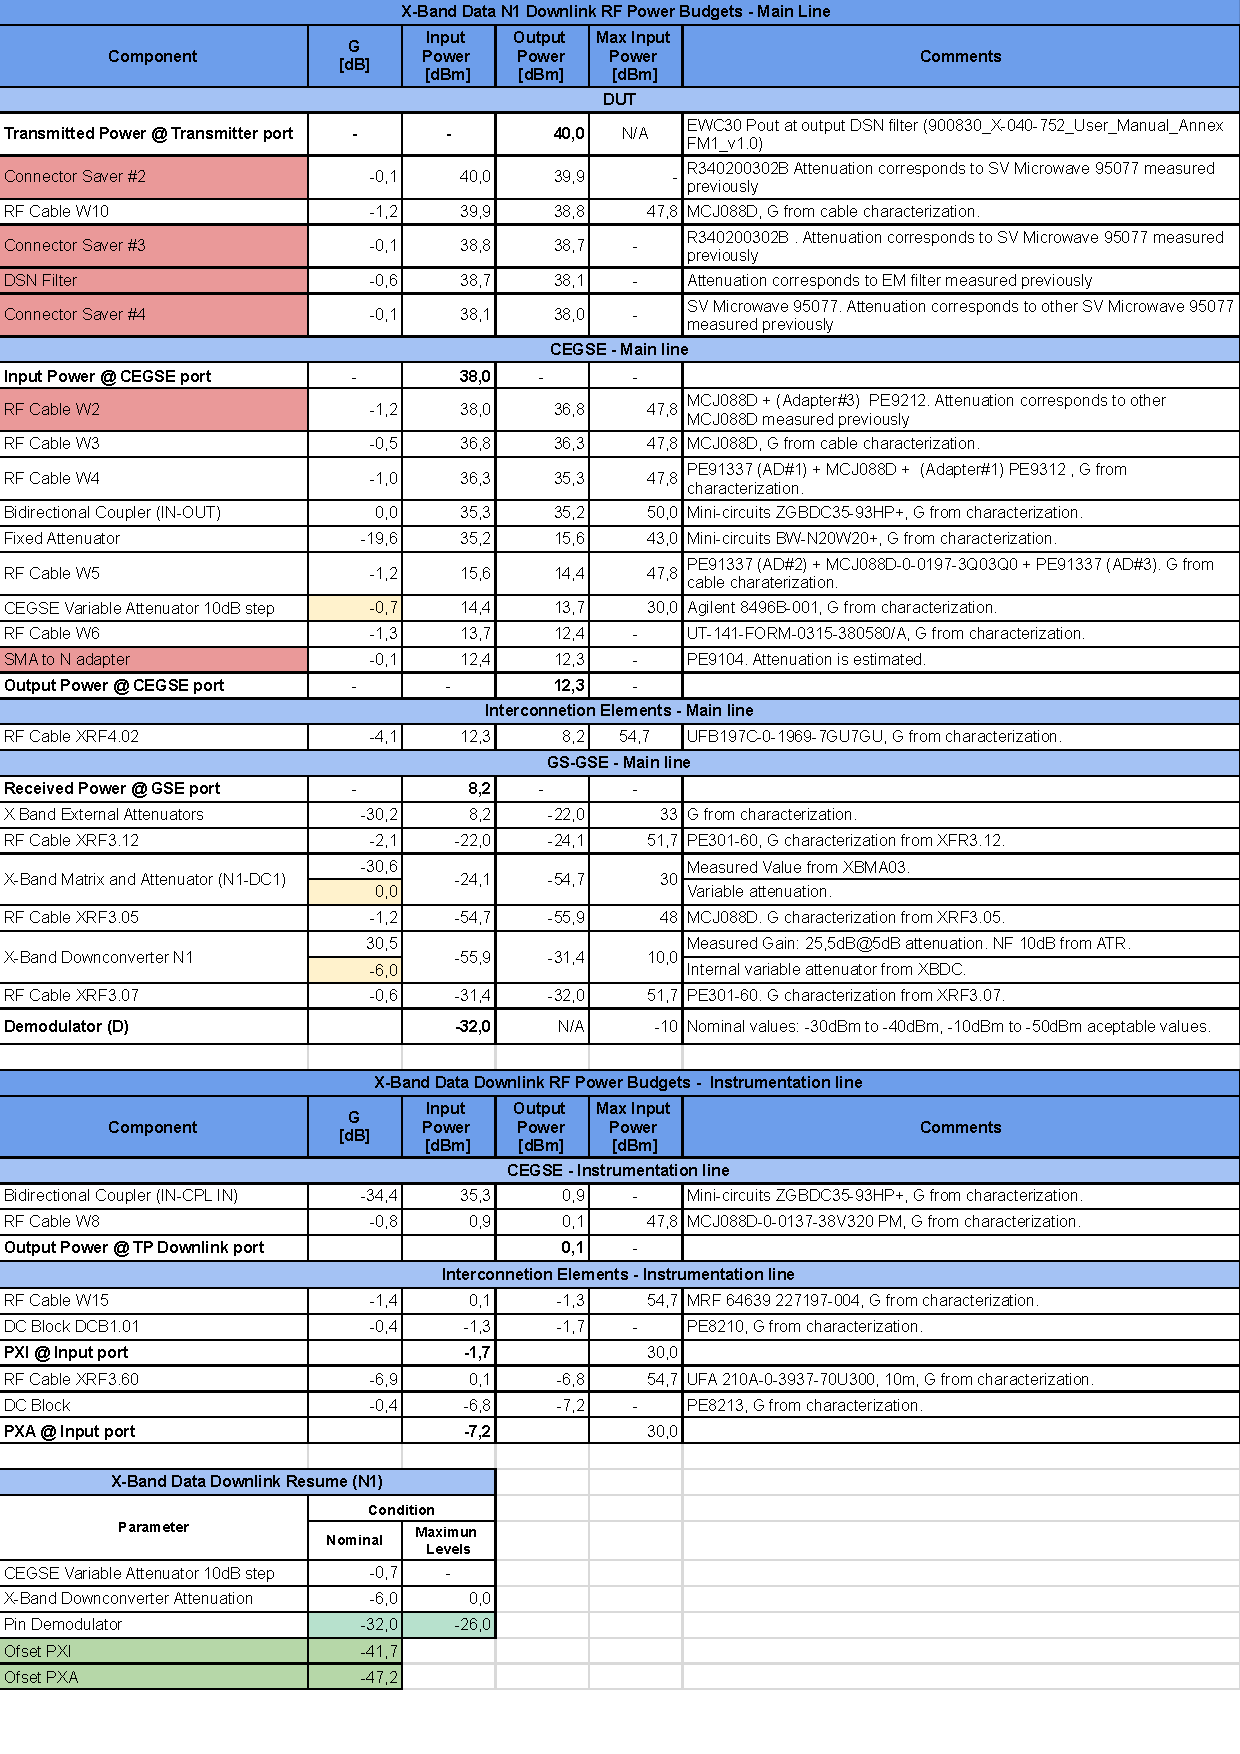
\includegraphics[page=1, scale=0.75, trim=0cm 0cm 0cm 0cm, clip ]
	{tables/Ensayos COMM-SS Link Budget - X-Band Data N1 Downlink.pdf}\\
\end{table}

\begin{table}[H]
	\centering
	\caption{EWC30-FM2 Link Budget - X-Band Data Downlink - case 1.} \label{tb:Data_DWL2}
	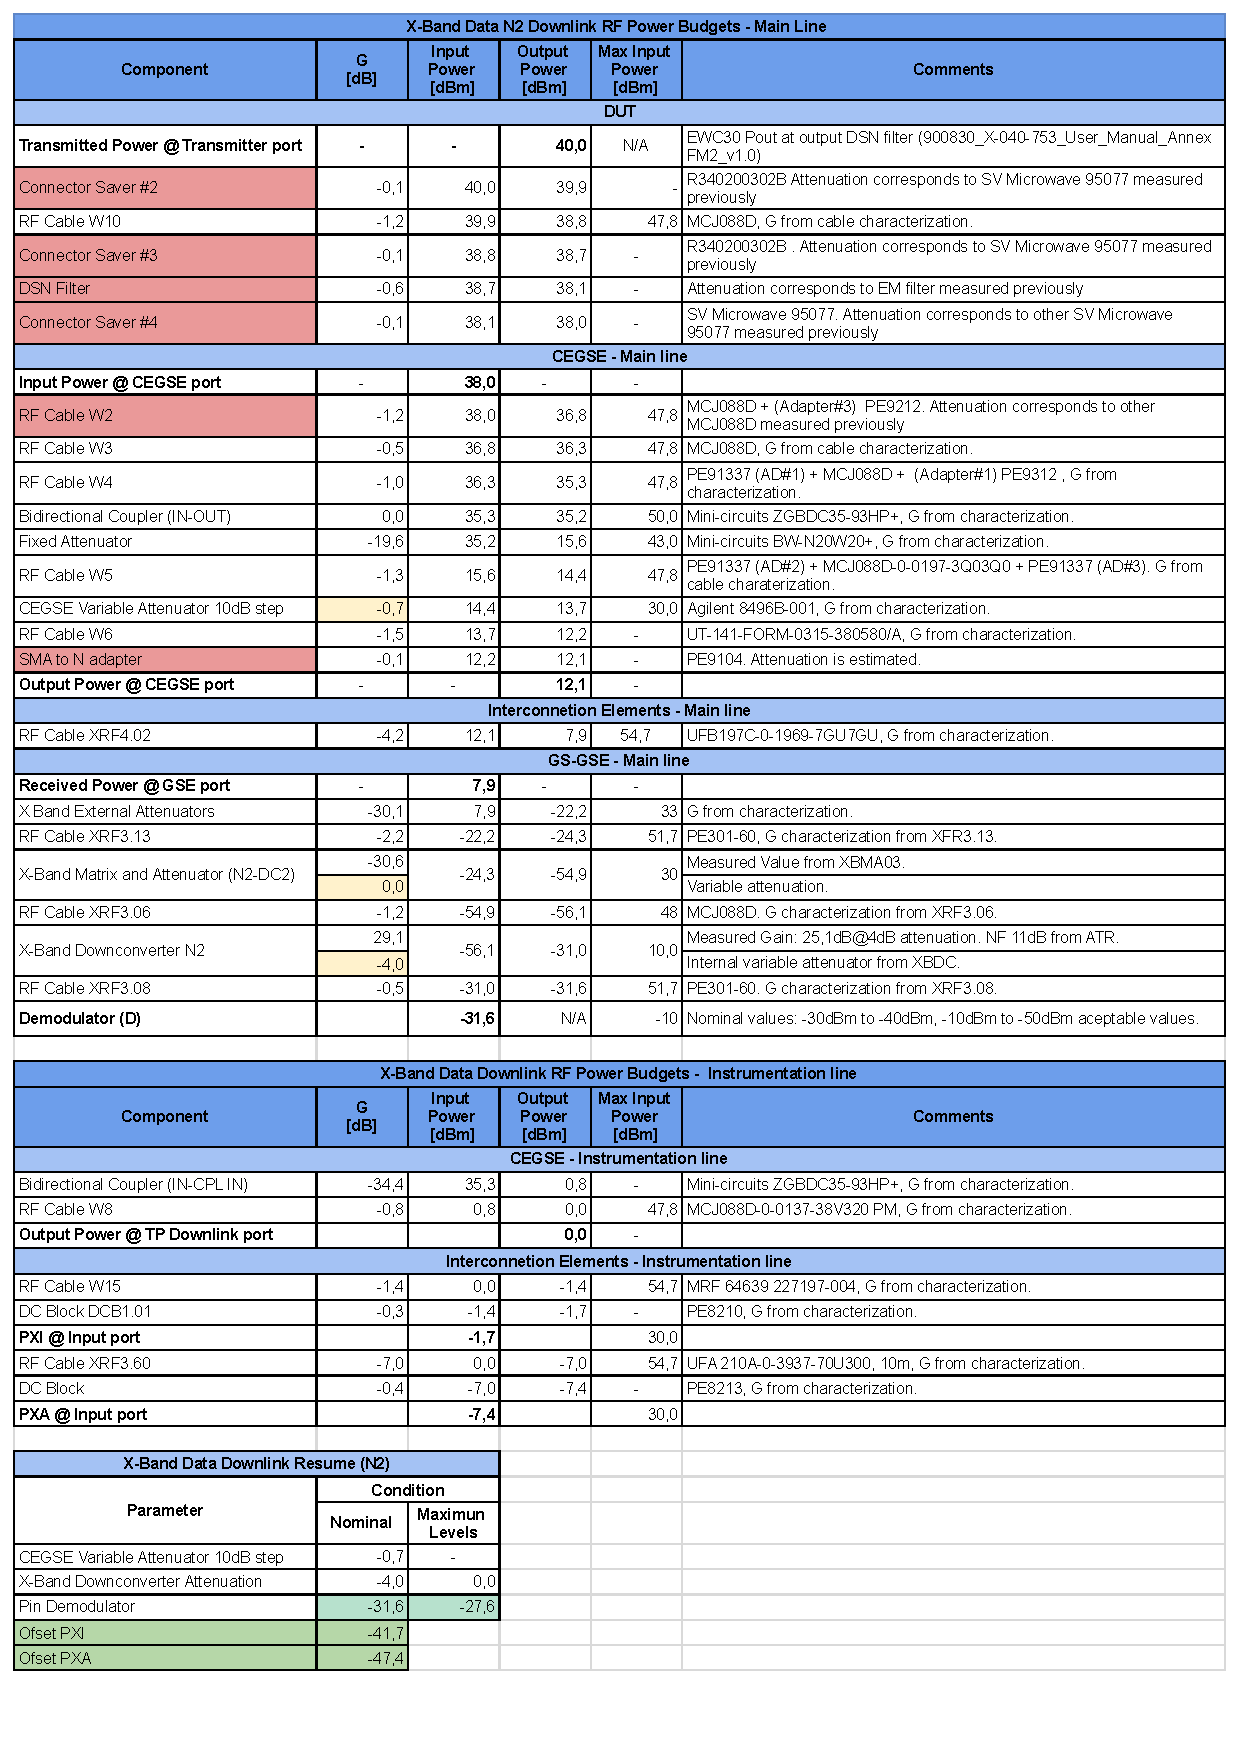
\includegraphics[page=1, scale=0.75, trim=0cm 0cm 0cm 0cm, clip ]
	{tables/Ensayos COMM-SS Link Budget - X-Band Data N2 Downlink.pdf}\\
\end{table}

\begin{table}[H]
	\centering
	\caption{EWC30-FM1 Link Budget - X-Band Data Downlink - case 2.} \label{tb:Data_EBN0FM1}
	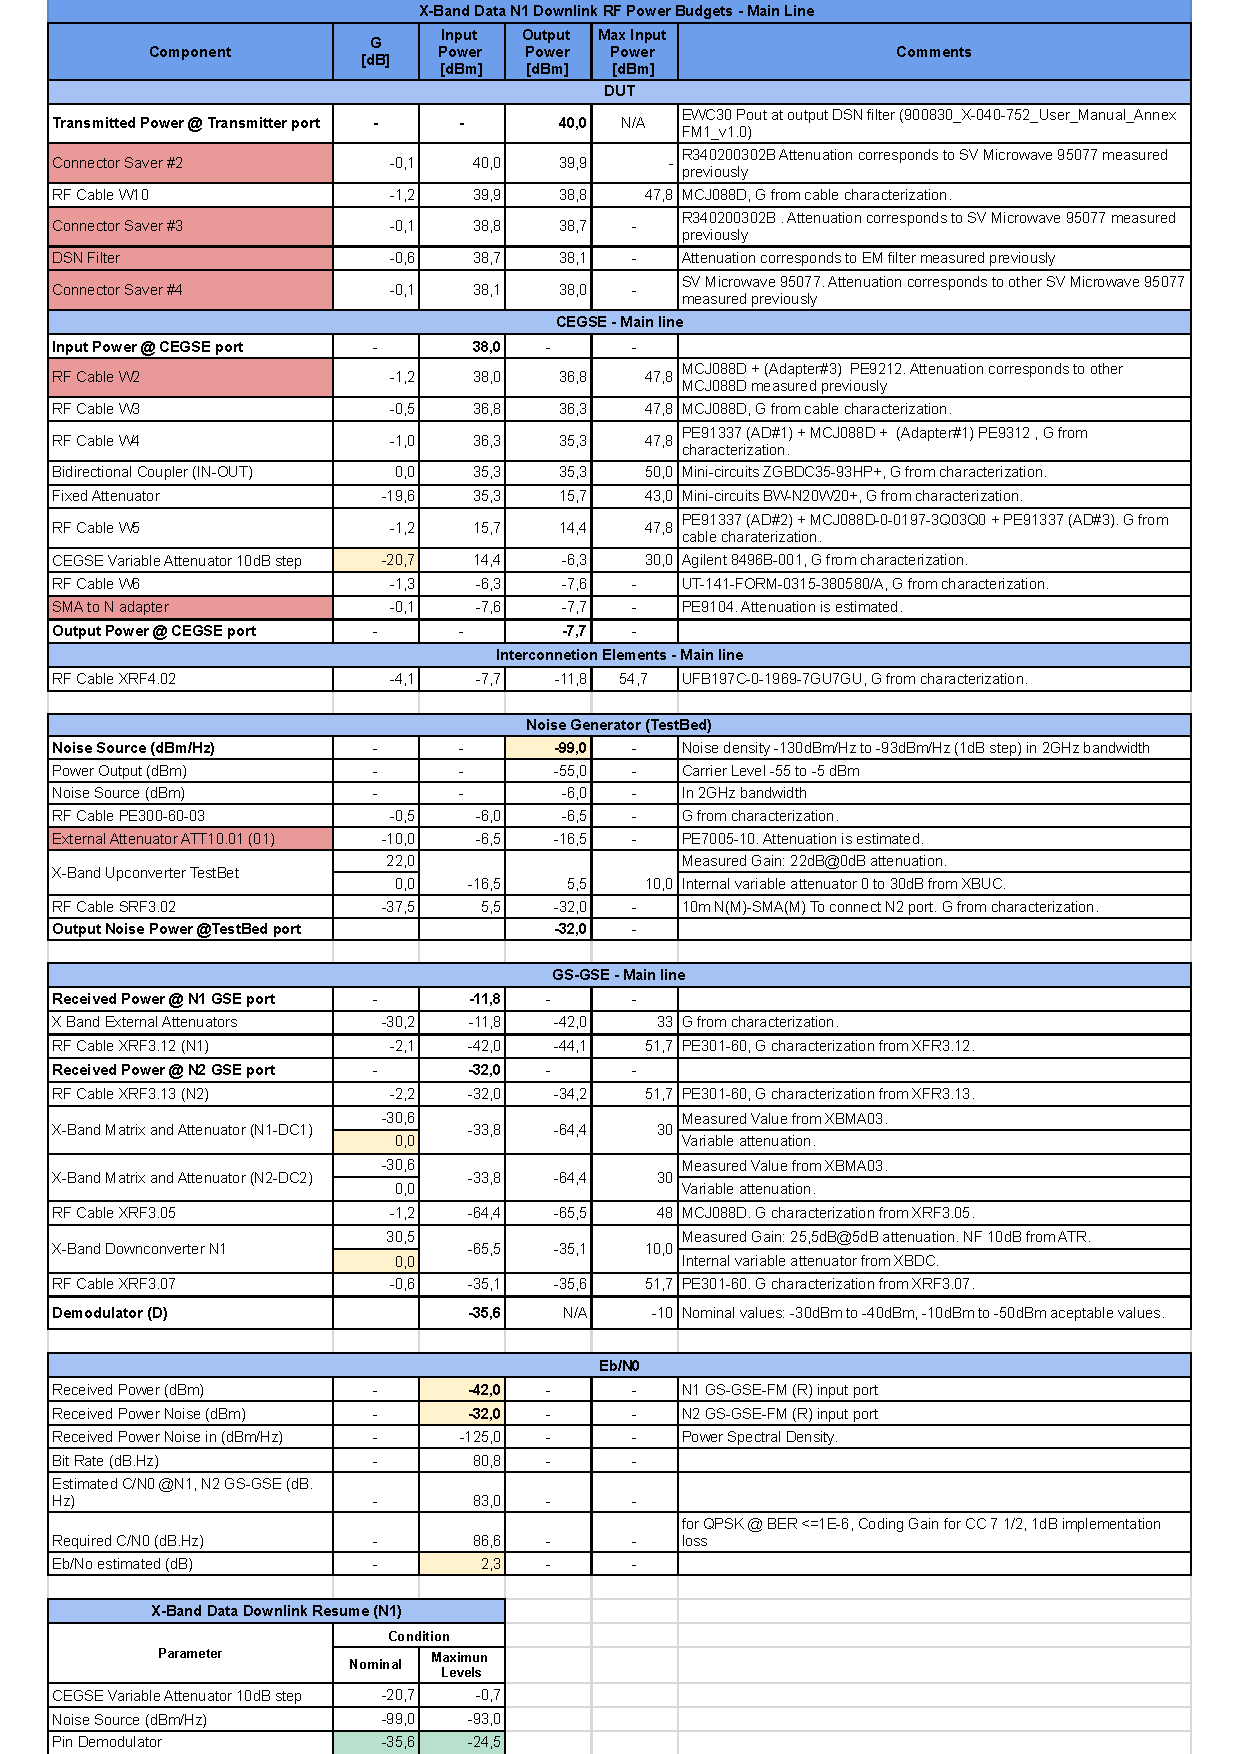
\includegraphics[page=1, scale=0.75, trim=0cm -0.3cm 0cm 0cm, clip ]
	{tables/Ensayos COMM-SS Link Budget -EBN0 X-Band Data N1 Downlink.pdf}\\
\end{table}

\begin{table}[H]
	\centering
	\caption{EWC30-FM2 Link Budget - X-Band Data Downlink - case 2.} \label{tb:Data_EBN0FM2}
	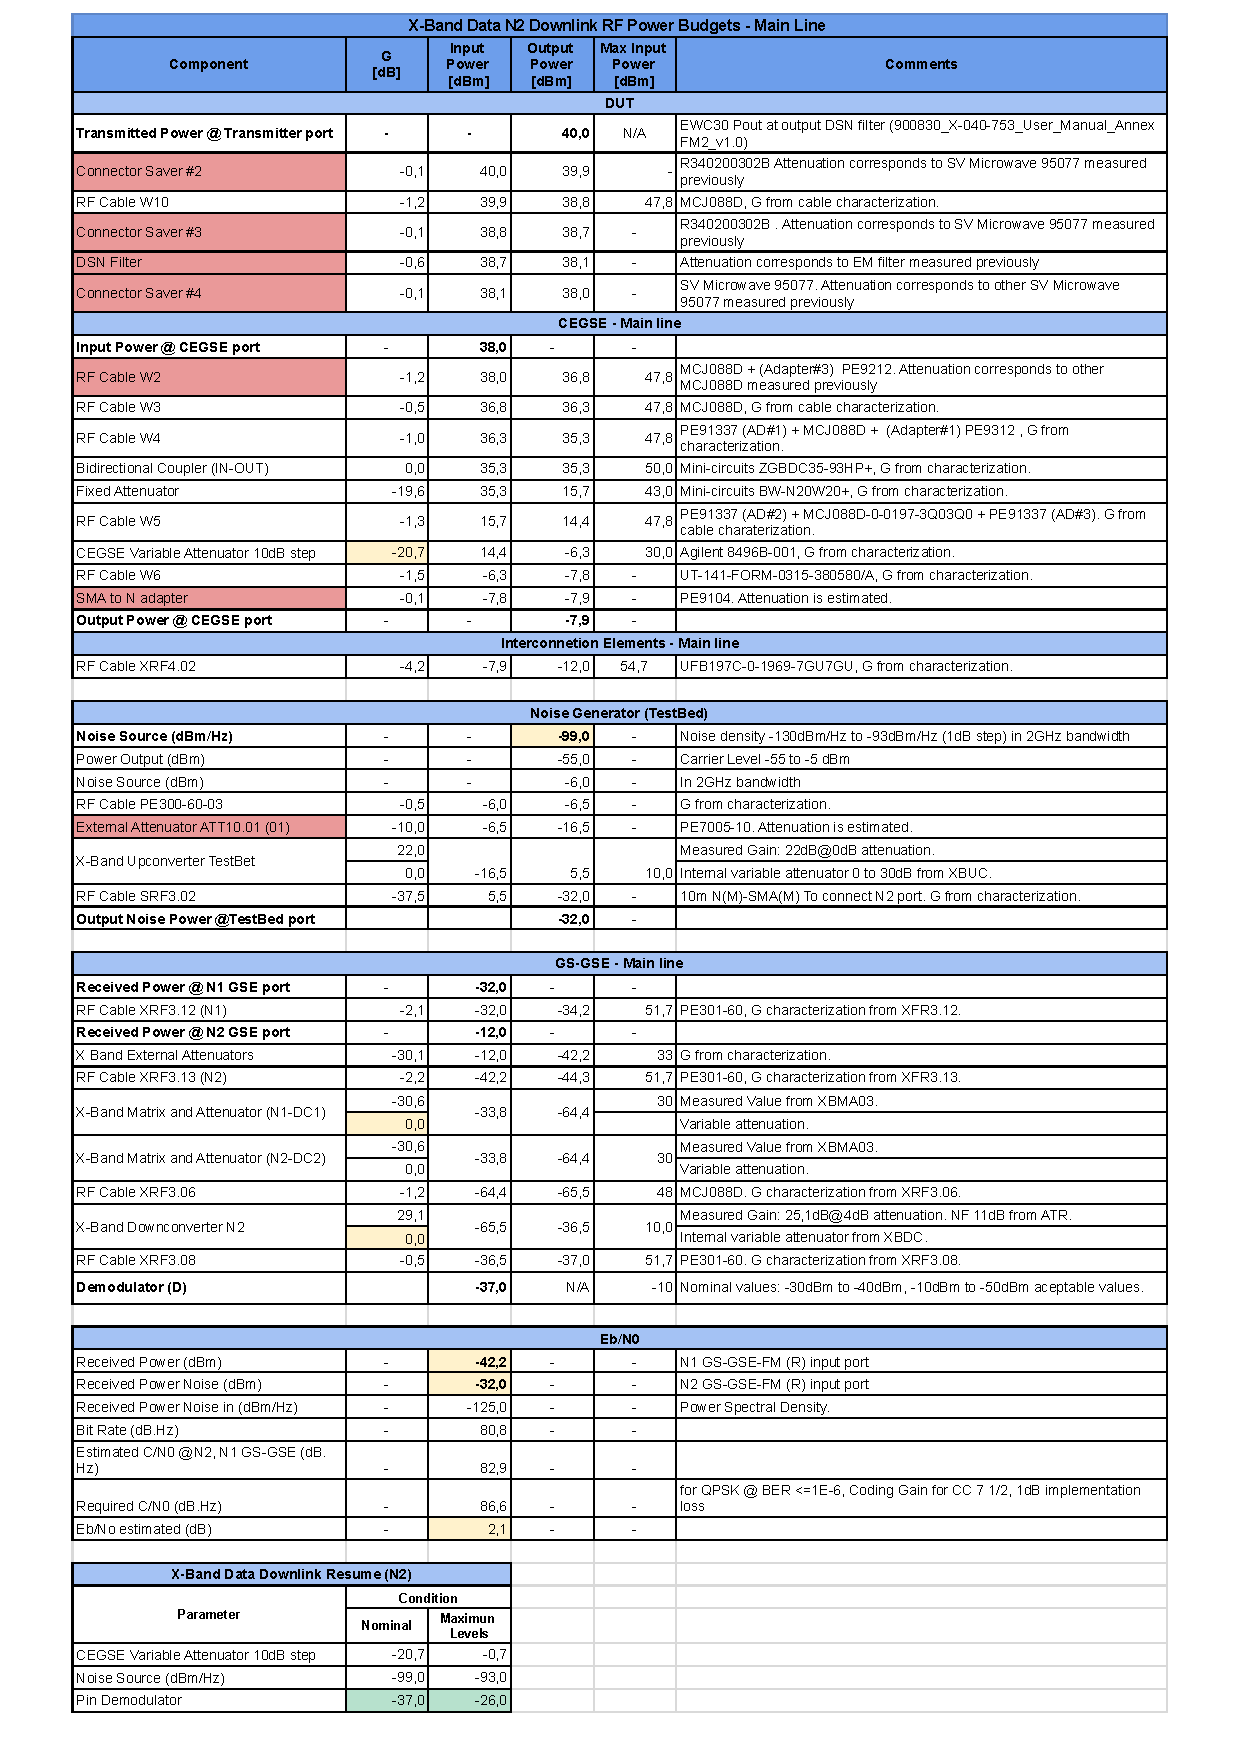
\includegraphics[page=1, scale=0.75, trim=0cm 0cm 0cm 0cm, clip ]
	{tables/Ensayos COMM-SS Link Budget -EBN0 X-Band Data N2 Downlink.pdf}\\
\end{table}

\begin{table}[H]
	\centering
	\caption{EWC30-FM1 Link Budget - X-Band Data Downlink - case 3.} \label{tb:Data_DSNFM1}
	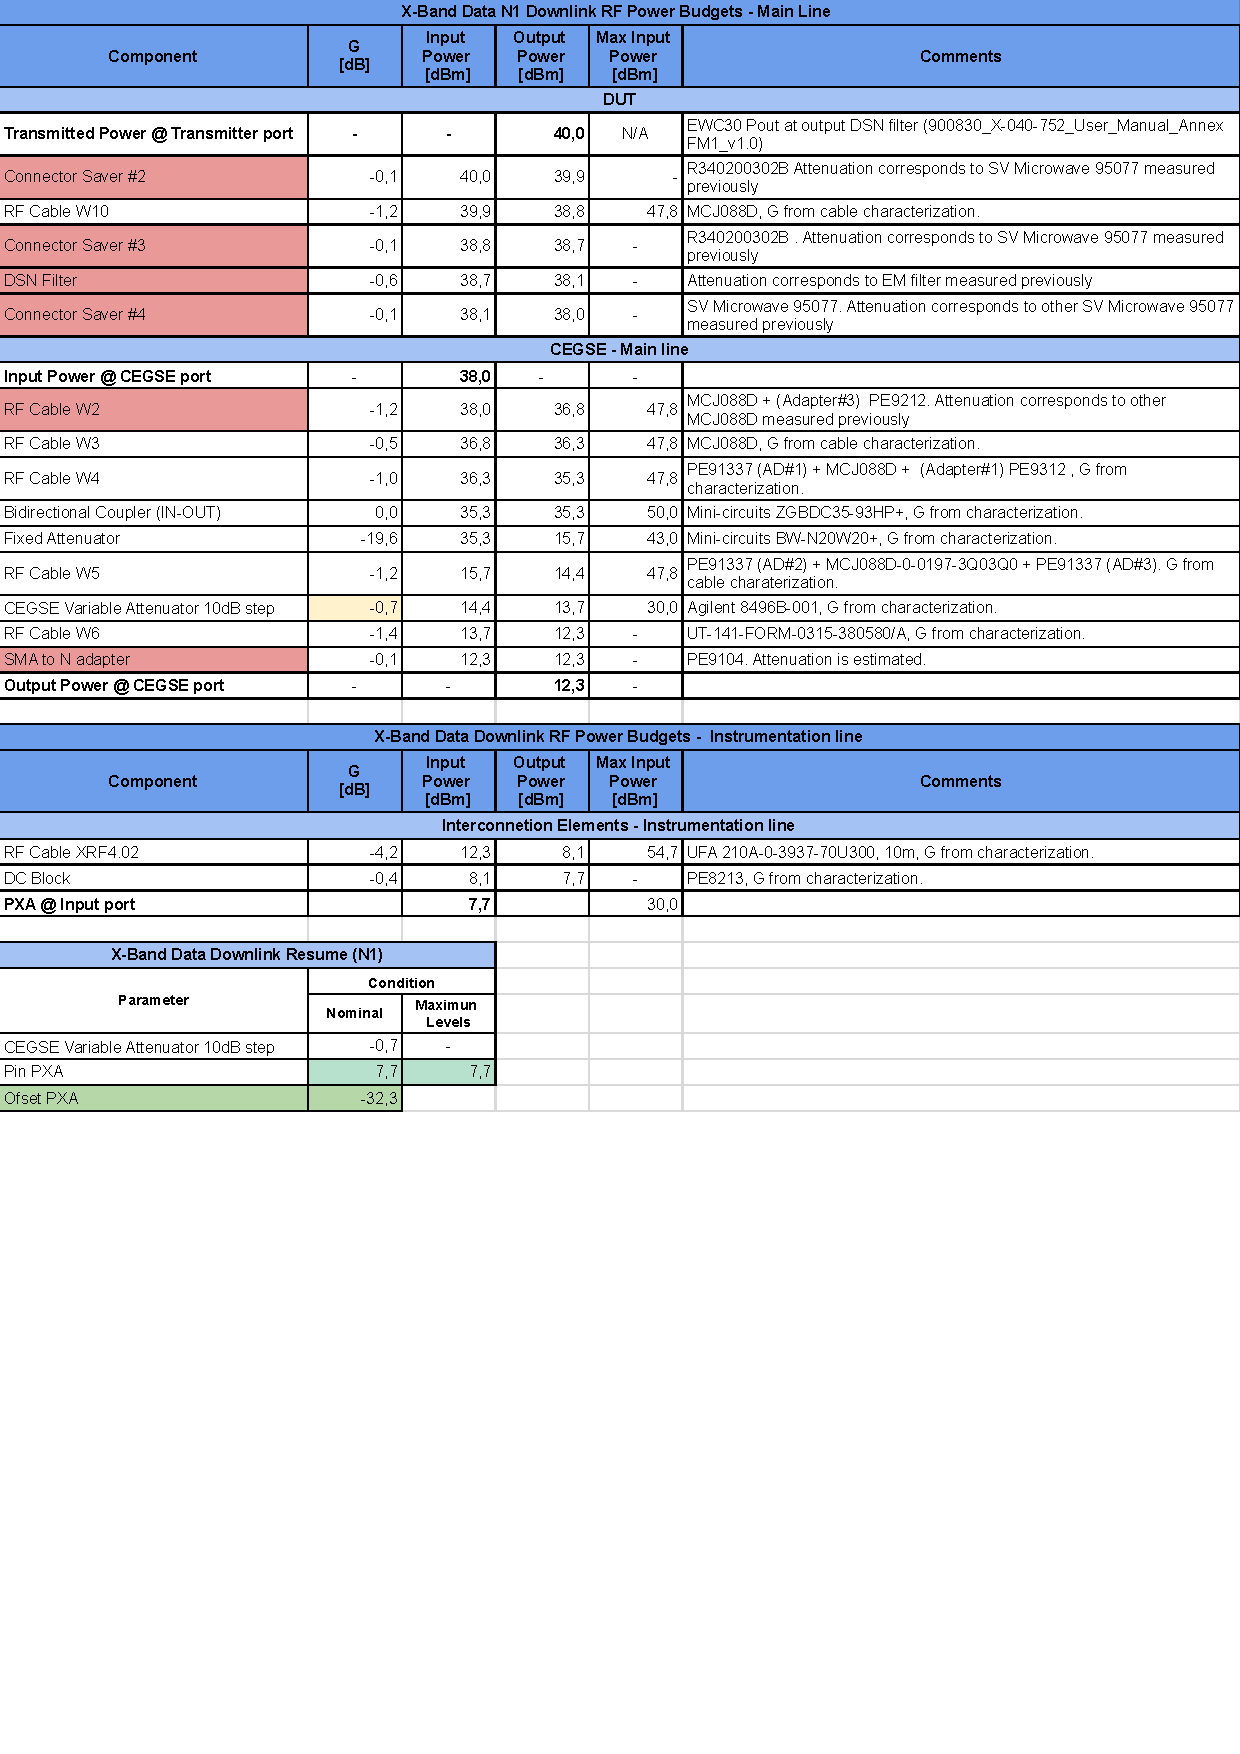
\includegraphics[page=1, scale=0.75, trim=0cm -0.3cm 0cm 0cm, clip ]
	{tables/Ensayos COMM-SS Link Budget -DSN X-Band Data N1 Downlink.pdf}\\
\end{table}

\begin{table}[H]
	\centering
	\caption{EWC30-FM2 Link Budget - X-Band Data Downlink - case 3.} \label{tb:Data_DSNFM2}
	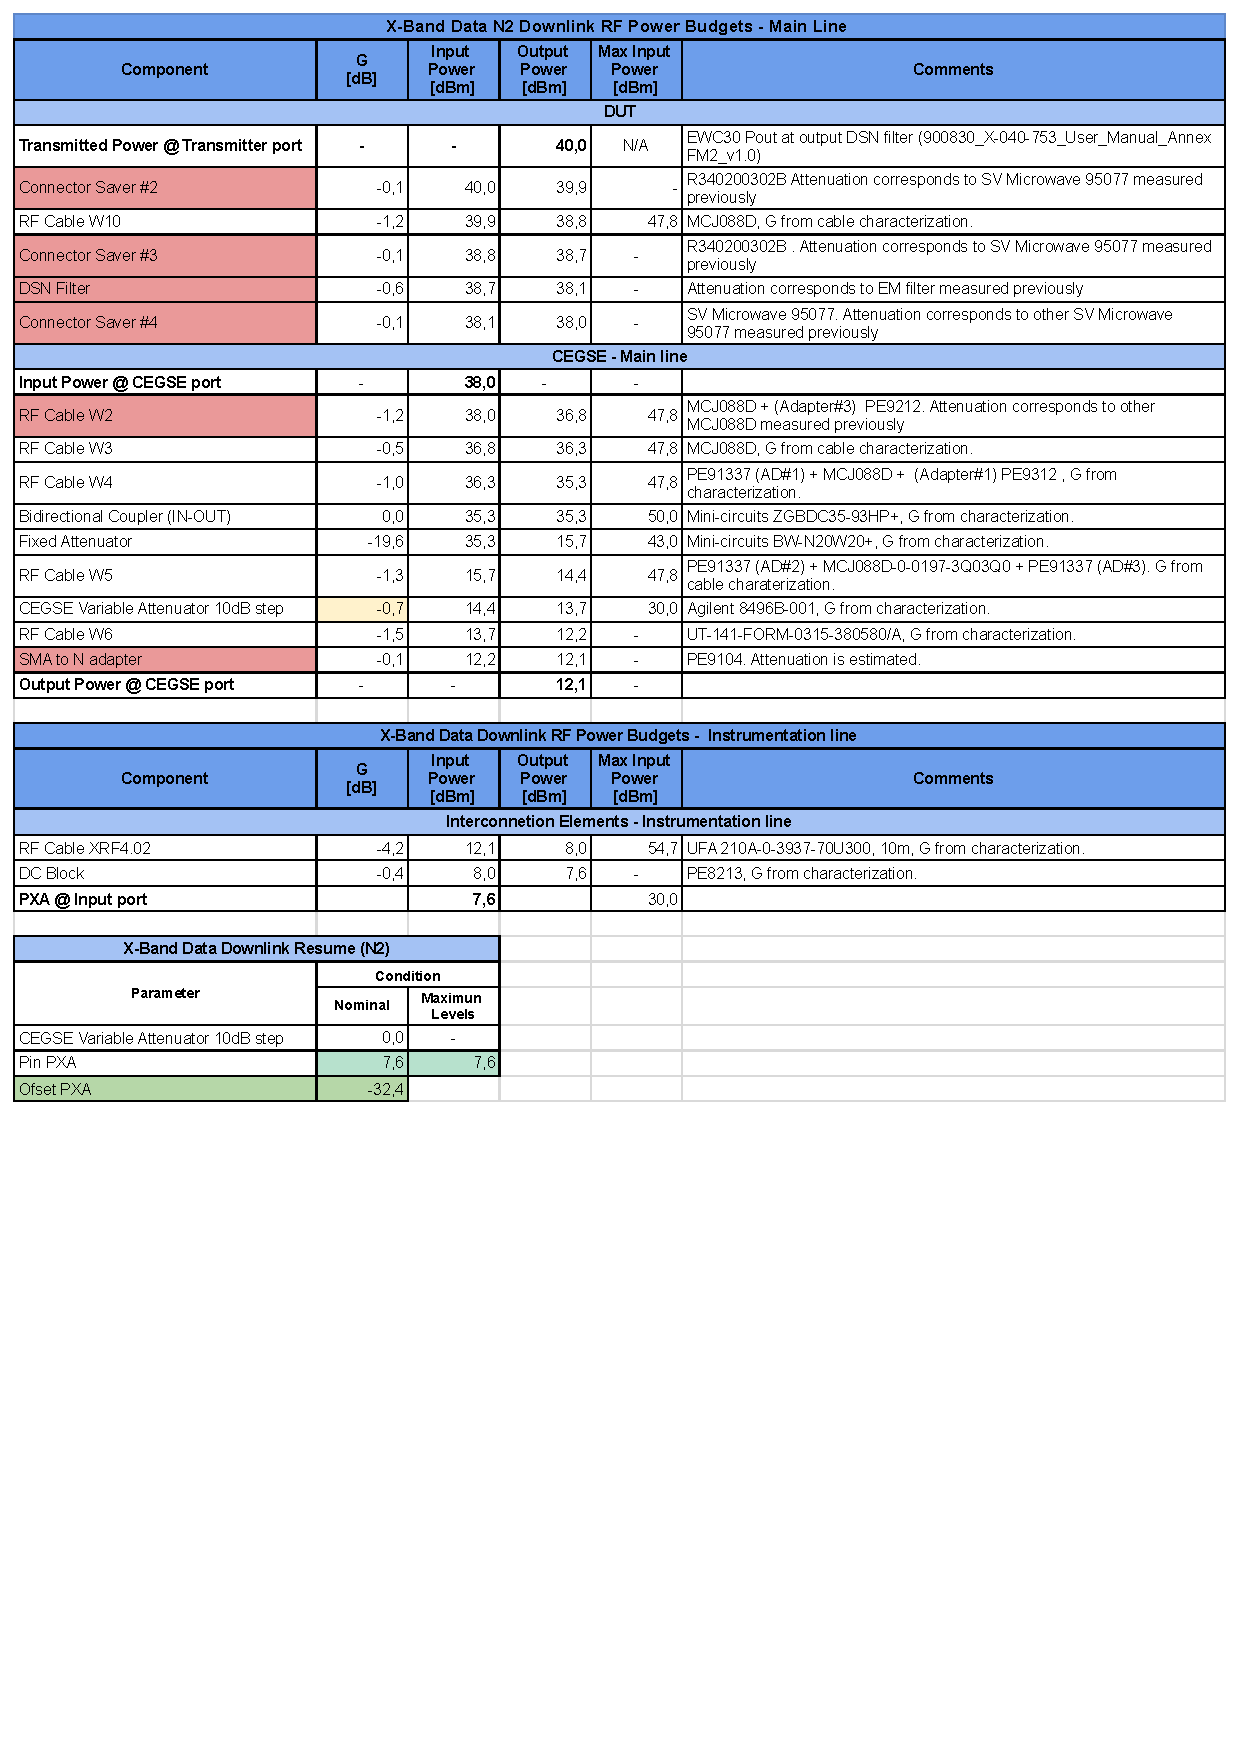
\includegraphics[page=1, scale=0.75, trim=0cm 0cm 0cm 0cm, clip ]
	{tables/Ensayos COMM-SS Link Budget -DSN X-Band Data N2 Downlink.pdf}\\
\end{table}